% ------------------------------------------------------------------------------
% TYPO3 Version 10.3 - What's New (German Version)
%
% @license	Creative Commons BY-NC-SA 3.0
% @link		https://typo3.org/help/documentation/whats-new/
% @language	German
% ------------------------------------------------------------------------------

\section{Datenschutz und Sicherheit}
\begin{frame}[fragile]
	\frametitle{Datenschutz und Sicherheit}

	\begin{center}\huge{Kapitel 5:}\end{center}
	\begin{center}\huge{\color{typo3darkgrey}\textbf{Datenschutz und Sicherheit}}\end{center}

\end{frame}

% ------------------------------------------------------------------------------
% Feature | 90333 | Dashboard

\begin{frame}[fragile]
	\frametitle{Datenschutz und Sicherheit}
	\framesubtitle{Dashboard}

	\begin{itemize}
		\item Dashboard-Widgets enthalten möglicherweise sensible Informationen.
		\item Wir empfehlen daher, Zugriffsberechtigungen für Widgets auf Gruppenbasis zu definieren.
		\item Backend-Benutzer haben nur Zugriff auf die Widgets, die für sie verfügbar sind.
		\item Benutzer mit Administratorberechtigungen haben immer Zugriff auf alle Widgets.
	\end{itemize}

\end{frame}

% ------------------------------------------------------------------------------
% Feature | 89978 | Introduce Status Report for insecure exception handler settings

\begin{frame}[fragile]
	\frametitle{Datenschutz und Sicherheit}
	\framesubtitle{Statusberichte}

	\begin{itemize}
		\item Der DebugExceptionHandler gibt möglicherweise sensible Daten aus, die
			zu einer Sicherheitslücke bei der Offenlegung von Informationen führen könnten.
		\item Ein neuer Statusbericht wurde eingefügt, um die Administratoren zu warnen.
	\end{itemize}

	\vspace{0.4cm}
	\textbf{WARNING}, wenn der Kontext auf \textbf{Entwicklung} eingestellt ist und die Fehlerausgabe aktiviert ist:
	\begin{figure}
		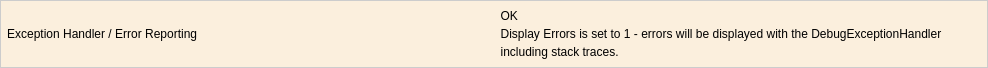
\includegraphics[width=1\linewidth]{SecurityAndPrivacy/89978a-IntroduceStatusReportForInsecureExceptionHandlerSettings.png}
	\end{figure}

	\textbf{ERROR}, wenn der Kontext auf \textbf{Produktion} gesetzt ist:
	\begin{figure}
		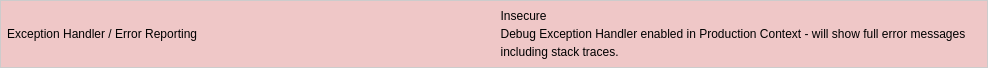
\includegraphics[width=1\linewidth]{SecurityAndPrivacy/89978b-IntroduceStatusReportForInsecureExceptionHandlerSettings.png}
	\end{figure}

\end{frame}

% ------------------------------------------------------------------------------
% Feature | 90351 | Allow TYPO3 to make SameSite cookies configurable

\begin{frame}[fragile]
	\frametitle{Datenschutz und Sicherheit}
	\framesubtitle{SameSite-Cookies (1)}

	\begin{itemize}
		\item Um den Datenschutz und die Sicherheit zu stärken, unterstützt TYPO3 nun die "SameSite"-Option
			für Cookies, die vom TYPO3-Kern gesetzt werden.
		\item Das Attribut wird von den meisten modernen Browsern unterstützt und ermöglicht es Websites
			zu erklären, ob Cookies eingeschränkt werden sollen.
		\item Laut
			\href{https://www.owasp.org/index.php/SameSite}{OWASP} mindern SameSite-Cookies\newline
			\small
				"\textit{das Risiko der Durchsickerung von Informationen aus verschiedenen Quellen}", mit\newline
				"\textit{einem gewissen Schutz von Cross-Site-Request-Fälschungsangriffen}".
			\normalsize

		\item Gültige Eistellungen sind "\textbf{strict}", "\textbf{lax}", oder \textit{not set}.
	\end{itemize}

\end{frame}

% ------------------------------------------------------------------------------
% Feature | 90351 | Allow TYPO3 to make SameSite cookies configurable

\begin{frame}[fragile]
	\frametitle{Datenschutz und Sicherheit}
	\framesubtitle{SameSite-Cookies (2)}

	\begin{itemize}
		\item TYPO3 setzt die folgenden Optionen:

			\begin{itemize}\small
				\item FE-User Sessions: "lax" by default
				\item BE-User Sessions: "strict" by default
				\item Install Tool Sessions: "strict" (nicht konfigurierbar)
				\item Last Login Provider (BE): "strict" (nicht konfigurierbar)
			\end{itemize}\normalsize

		\item Das Install Tool bietet eine Systemkonfiguration zur Anpassung der
			SameSite-Cookie-Richtlinien, wenn die Standardeinstellungen zu streng sind
			(z.B. bei Authentifizierungsanbietern wie OpenID/OAuth).

		\item Lesen Sie mehr über SameSite-Cookies in
			\href{https://tools.ietf.org/html/draft-ietf-httpbis-cookie-same-site-00}{RFC6265} (Entwurf).
	\end{itemize}

\end{frame}

% ------------------------------------------------------------------------------
% Feature | 90262 | Add Argon2id to password hash algorithms

\begin{frame}[fragile]
	\frametitle{Datenschutz und Sicherheit}
	\framesubtitle{Passwort-Hash-Algorithmen}

	\begin{itemize}
		\item Der Hashing-Algorithmus \texttt{Argon2i} ("i") wurde mit TYPO3 v9 LTS eingeführt.
		\item \texttt{Argon2id} ("id") ist jetzt auch in TYPO3 verfügbar, wenn die PHP-Version dies unterstützt.
		\item \texttt{Argon2id} ist ein Hybrid aus \texttt{Argon2i} und \texttt{Argon2d}
			und ist resistenter gegen Seitenkanal-Angriffe.
		\item \texttt{Argon2id} ist normalerweise auf Systemen mit PHP Version 7.3 oder höher verfügbar.
	\end{itemize}

\end{frame}

% ------------------------------------------------------------------------------
